\section{Procedure}
\label{sec:procedure}
The experiment consists of two parts. While in both parts the Hall voltage is being measured,
different paramters are varied. For both parts the setup is similar and the procedure is simplified
by having a computer to record the data.

\subsection{Measuring the Hall voltage as function of current}
\label{sec:procedure:a}
The wiring setup is shown in \autoref{fig:wiring}. Important here is the correct setup of the base
unit. Furthermore, the polarization of the magnetic coils need to be considered, such that the two
sides interfere constructively.

For the measurement itself, the software Cassy on the computer has to be used. In the software the
input data has to be set to the Hall voltage and the probe current and the recording shall be
started. Then you can manually increase the current. The measurement can be repeated with different
magnetic fields, which can be adjusted through the coil current.

\begin{figure}
  \centering
  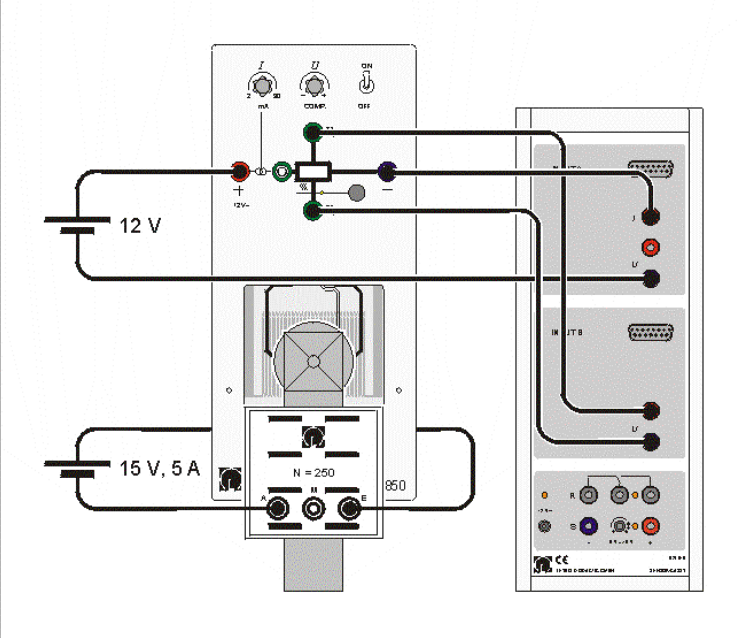
\includegraphics[width=0.4\textwidth]{media/wiring.png}
  \caption{Experimental setup (wiring diagram) for measuring the Hall
            voltage as function of the current I \cite{leaflet}.}
  \label{fig:wiring}
\end{figure}

\subsection{Measuring the Hall voltage as function of magnetic
field}
\label{sec:procedure:b}
For the second part the procedure is similar, except now the sample current is held constant and the
external magnetic field is the variable parameter. The main difference lies in the circuit. Instead
of connecting the sample current to the upper input (input A) in \autoref{fig:wiring}, one has to
connect the magnetic field probe. 

The recording procedure is similar, except that now the coil current has to be continuously moved
from $\SI{0}{A}$ to $\SI{5}{A}$.

\subsection{Compensation of the Hall Voltage}
\label{sec:compensation}
Eventhough we did not have to perform this part, sometimes a compensation has to be interoduced.
This shifts the Hall voltage in such a way that it is $\SI{0}{V}$ when the magnetic field is
$\SI{0}{B}$. To do so, on measures $U_\text{H}$ with a maximal cross current and no magnetic field.
The measuring unit has a turn dial which can be turned until the is no Hall voltage.

